

\documentclass[conference]{IEEEtran}
\IEEEoverridecommandlockouts
% The preceding line is only needed to identify funding in the first footnote. If that is unneeded, please comment it out.
\usepackage{cite}
\usepackage{amsmath,amssymb,amsfonts}
\usepackage{algorithmic}
\usepackage{graphicx}
\usepackage{textcomp}
\usepackage{xcolor}
\def\BibTeX{{\rm B\kern-.05em{\sc i\kern-.025em b}\kern-.08em
    T\kern-.1667em\lower.7ex\hbox{E}\kern-.125emX}}
\begin{document}

\title{SMART TIFFIN BOX\\
\author{\IEEEauthorblockN{Md Firose Mahmud (munna003.bubt@gmail.com)\IEEEauthorrefmark{1},
Partho Debnath\IEEEauthorrefmark{2},
Md Arafat Hossan\IEEEauthorrefmark{3}, \\
Mohammad Ali\IEEEauthorrefmark{4}, Sanjana Islam\IEEEauthorrefmark{5}}

\IEEEauthorblockA{Student, Dept. of CSE\\Bangladesh University of Business and Technology, Bangladesh\\
\IEEEauthorrefmark{1}ID 19201103003,\IEEEauthorrefmark{2}ID 19201103016,\IEEEauthorrefmark{3}ID 19201103039\\\IEEEauthorrefmark{4}ID 19201103006,\IEEEauthorrefmark{5}ID 19201103021}

}


}



\maketitle

\begin{abstract}
This report presents an Internet of Things (IoT) based project for a SMART Tiffin Box. The project is aimed at providing users with an automated solution to their daily tiffin box needs. The system consists of three interconnected components: a Node MCU-based circuit, an Android app and an Arduino cloud-based web service. The Node MCU-based circuit is used to detect the temperature of the tiffin box and control a servo motor to connect the heat generator coil with power source. The Android app is used to control the motor, as well as to receive the real time temperature of the tiffin box. Finally, the cloud-based web service is used to store and process data related to the tiffin box. The project provides an efficient and reliable solution to the problem of providing users with a safe and automated way to controlling food temperature of a tiffin box.
\end{abstract}

\begin{IEEEkeywords}
 NodeMCU, Arduino Cloud, Temperature Sensor, Heat Generator Coil
\end{IEEEkeywords}

\section{Introduction}
\textbf{Overview:} The SMART Tiffin Box is an IoT-based project that uses advanced technology to provide convenience, security, and health benefits to users. The project utilizes cutting-edge sensors and communication technologies to monitor food temperature. The SMART Tiffin Box also comes with an integrated mobile app that allows users to remotely control and monitor the system from anywhere. Through the app, user can check the temperature and to increase food temperature press the button for on the heat generator coil. Beside user control, our system can control it when the temperature up to a fixed value. The SMART Tiffin Box is a great solution for busy people who need to eat hot food in a office, school, college and so on. \\\\
\textbf{Purpose:} Most of the time we use tiffin box to carry food and once time the food gets cold. To maintaining the food temperature using android app from anywhere. We have tried to focus on food temperature just. This is a user-friendly project for the android app, free Arduino Cloud system for storage. 

\section{Literature Survey}

\textbf{Existing Problem:\\} Food safety is a major concern for our health, and proper temperature control is critical in ensuring the safety of the food. The traditional methods of temperature monitoring and regulation, such as manual measurements and adjusting the heating elements of food, are time-consuming, prone to errors, and may not provide real-time alerts when the temperature exceeds the safe range. \\
\textbf{Proposed Solution:\\}Temperature is a critical factor for ensuring the safety and quality of fresh and healthy food. Proper temperature control can prevent the growth of harmful bacteria and other microorganisms, as well as slow down the chemical and enzymatic reactions that can lead to spoilage.
The "SMART Tiffin Box" project is an IoT-based system that aims to provide users with a convenient way to monitor and control the temperature of their food. The system consists of a temperature sensor that is placed inside the food container, which constantly senses the temperature of the food and sends the data to the user's mobile app via an Arduino cloud-based server.\\
Using the app, the user can monitor the temperature of their food in real-time. The app also allows the user to remotely control the heating elements of the food container to maintain the optimal temperature for the food.
By using the SMART Tiffin Box, users can ensure that they are eating healthy food that is cooked to the right temperature, reducing the risk of foodborne illnesses. The system is easy to use and can be used anywhere, making it ideal for busy individuals who want to stay healthy while on-the-go.


\section{Theoretical Analysis}
\textbf{Block Diagram:\\}

\begin{figure}[htbp]
\centerline{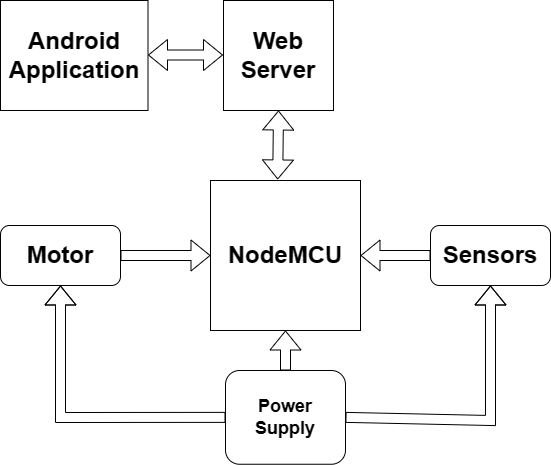
\includegraphics[width=0.3\textwidth]{blockdiagram.drawio.png}}
\caption{System Block Diagram}
\label{fig}
\end{figure}

\textbf{Software Designing:\\}

\subsection{Arduino Cloud}\label{AA}

The Arduino IoT Cloud is a platform that allows anyone to create IoT projects, with a user-friendly interface, and an all-in-one solution for configuration, writing code, uploading and visualization. To use the Arduino IoT Cloud, a cloud compatible board is required. Arduino Cloud employs the latest security standards to ensure the safety of your projects and project data.
\begin{figure}[htbp]
\centerline{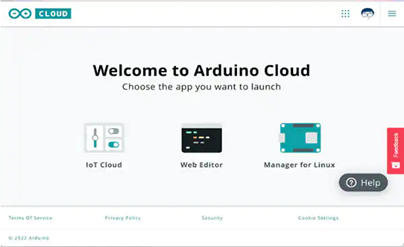
\includegraphics[width=0.4\textwidth]{Picture1.png}}
\caption{Arduino Cloud}
\label{fig}
\end{figure}
\\

\subsection{Arduino Cloud IDE}\label{AA}
This Web IDE is a part of Arduino Create, which is a platform for developers to write codes, access tutorials, configure boards and also share them to the world. This web IDE can also save your code on the cloud. In a nutshell, we can manage every aspect of our project online. The web editor of the Arduino Cloud offers the same functionality as the classic Arduino IDE. However, the web-based version allows you to work on your Arduino programs using different computers without copying files around or using a software configuration management (SCM) tool, such as GIT. The web IDE lets you edit sketches, import libraries, access the serial monitor, and compile and upload programs to your development boards.
\\\\\\
\begin{figure}[htbp]
\centerline{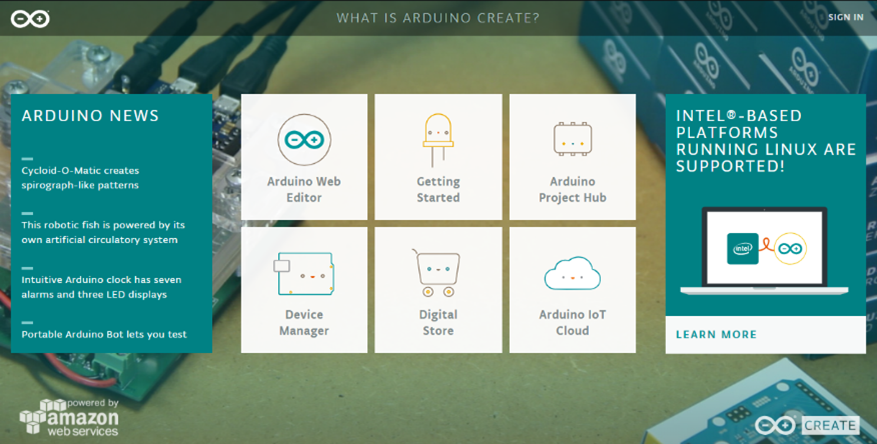
\includegraphics[width=0.4\textwidth]{Picture2.png}}
\caption{Arduino Cloud IDE}
\label{fig}
\end{figure}

\textbf{Hardware Designing:\\}
Here we used a NodeMCU controller, two power supply, DHT11 temperature sensor and a servo motor instead of switch.
\begin{figure}[htbp]
\centerline{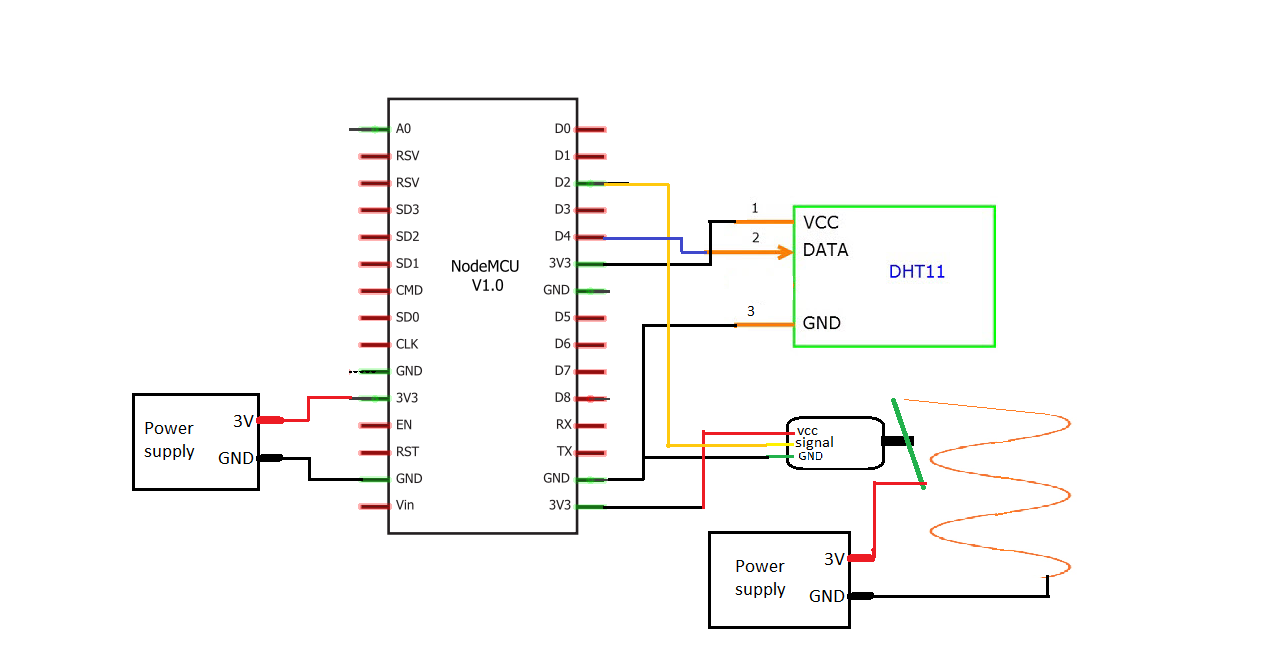
\includegraphics[width=0.5\textwidth]{Pin Diagram.png}}
\caption{Arduino Cloud IDE}
\label{fig}
\end{figure}


\section{Flowchart}
A Flowchart is a type of diagram used to represent a process or a workflow. Process flowcharts are visual representations of a step-by-step approach to arriving at a certain business outcome or solution to a given task. To illustrate the entire algorithmic process, the diagram employs various shapes and boxes describing attributes such as inputs/outputs, decisions, and comments, connected with a flowline showing the operation’s progress.

\begin{figure}[htbp]
\centerline{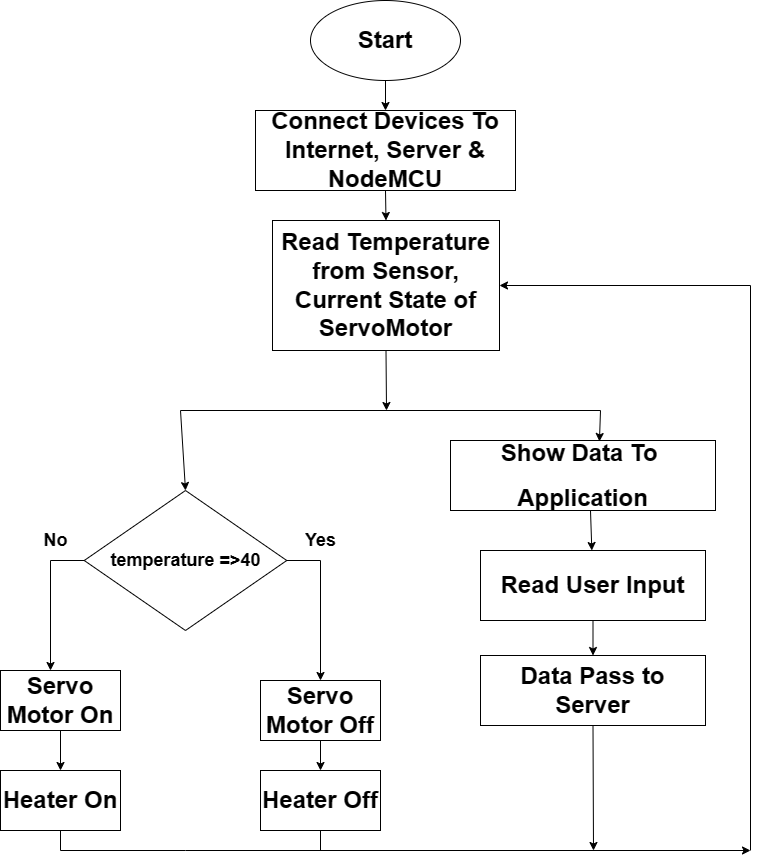
\includegraphics[width=0.5\textwidth]{Flow Chart.drawio (1).png}}
\caption{Flowchart of Proposed System}
\label{fig}
\end{figure}


\section{Results}

\begin{figure}[htbp]
\centerline{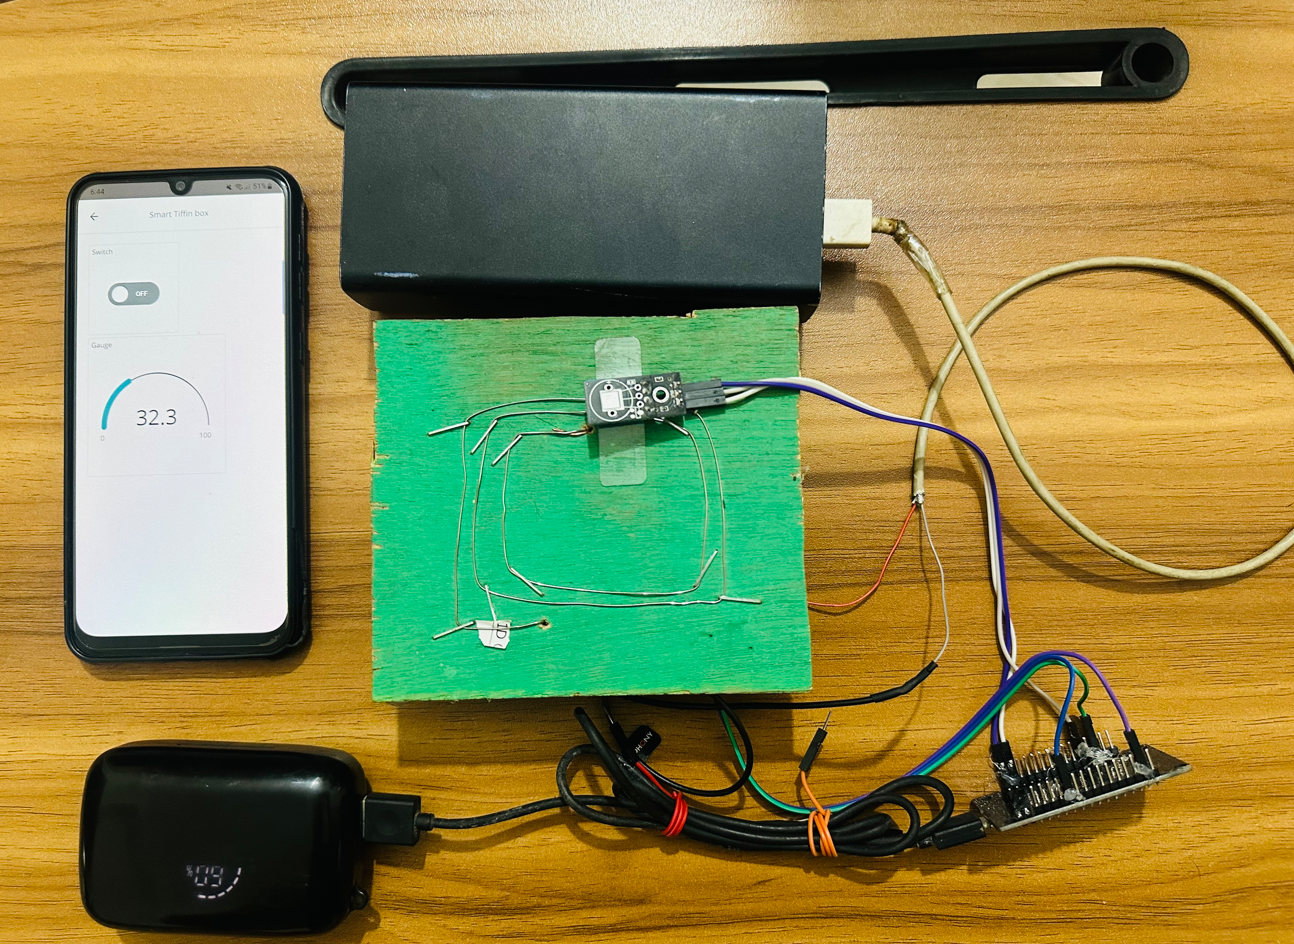
\includegraphics[width=0.5\textwidth, height=0.3\textwidth]{pic1.png}}
\caption{Normal Temperature}
\label{fig}
\end{figure}

\begin{figure}[htbp]
\centerline{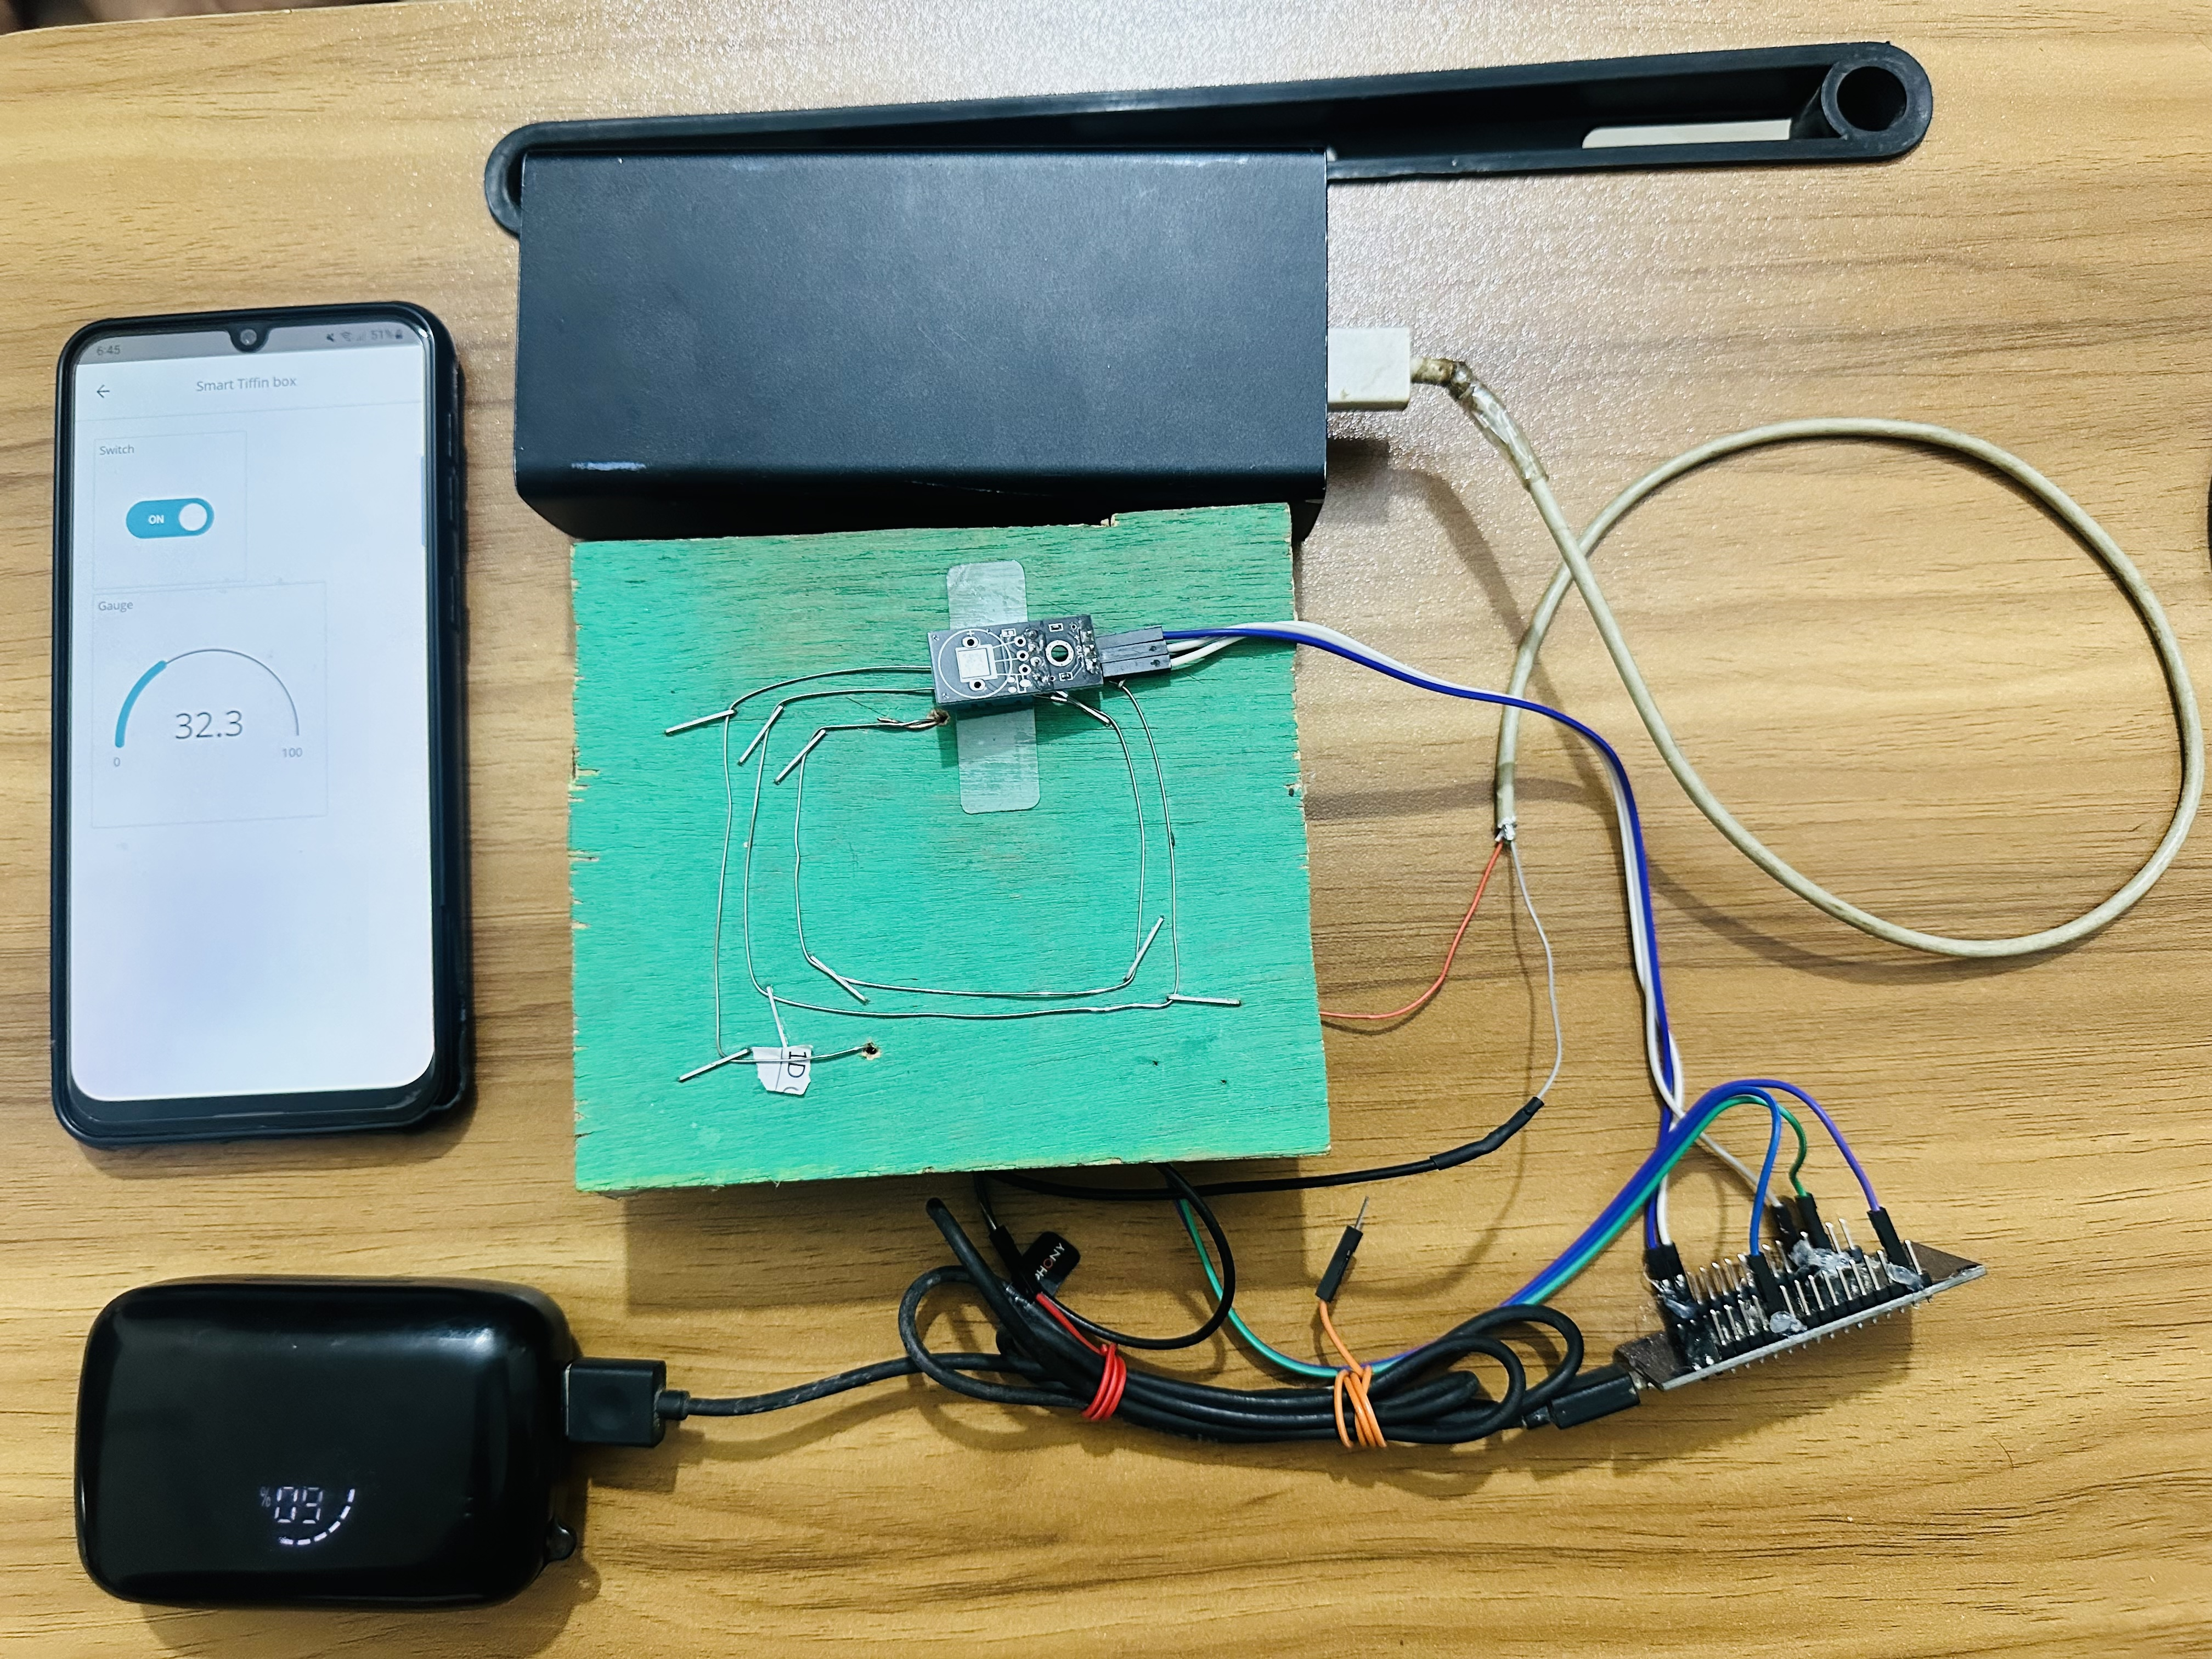
\includegraphics[width=0.5\textwidth, height=0.3\textwidth]{IMG_3503.jpg}}
\caption{Heat Generator Turn On}
\label{fig}
\end{figure}

\begin{figure}[htbp]
\centerline{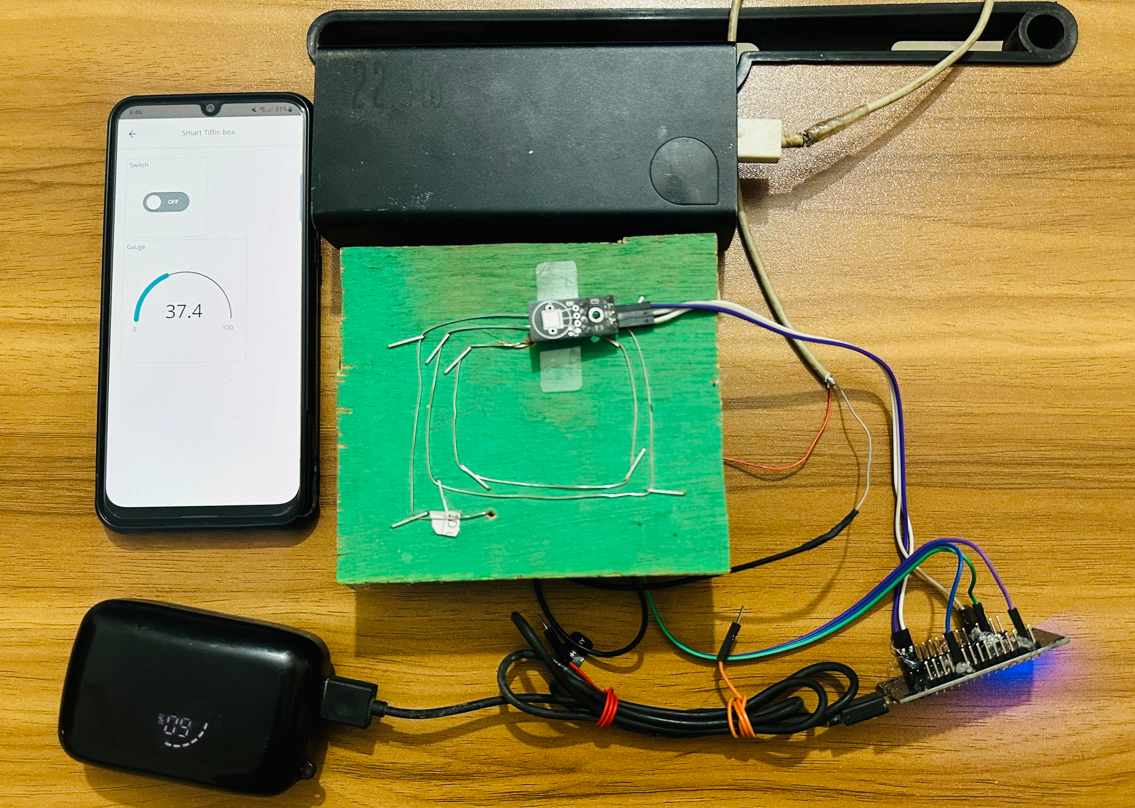
\includegraphics[width=0.5\textwidth, height=0.3\textwidth]{pic2.png}}
\caption{Auto Turn Off When Temp. Reach 37 Degree}
\label{fig}
\end{figure}
\newpage
\begin{figure}[htbp]
\centerline{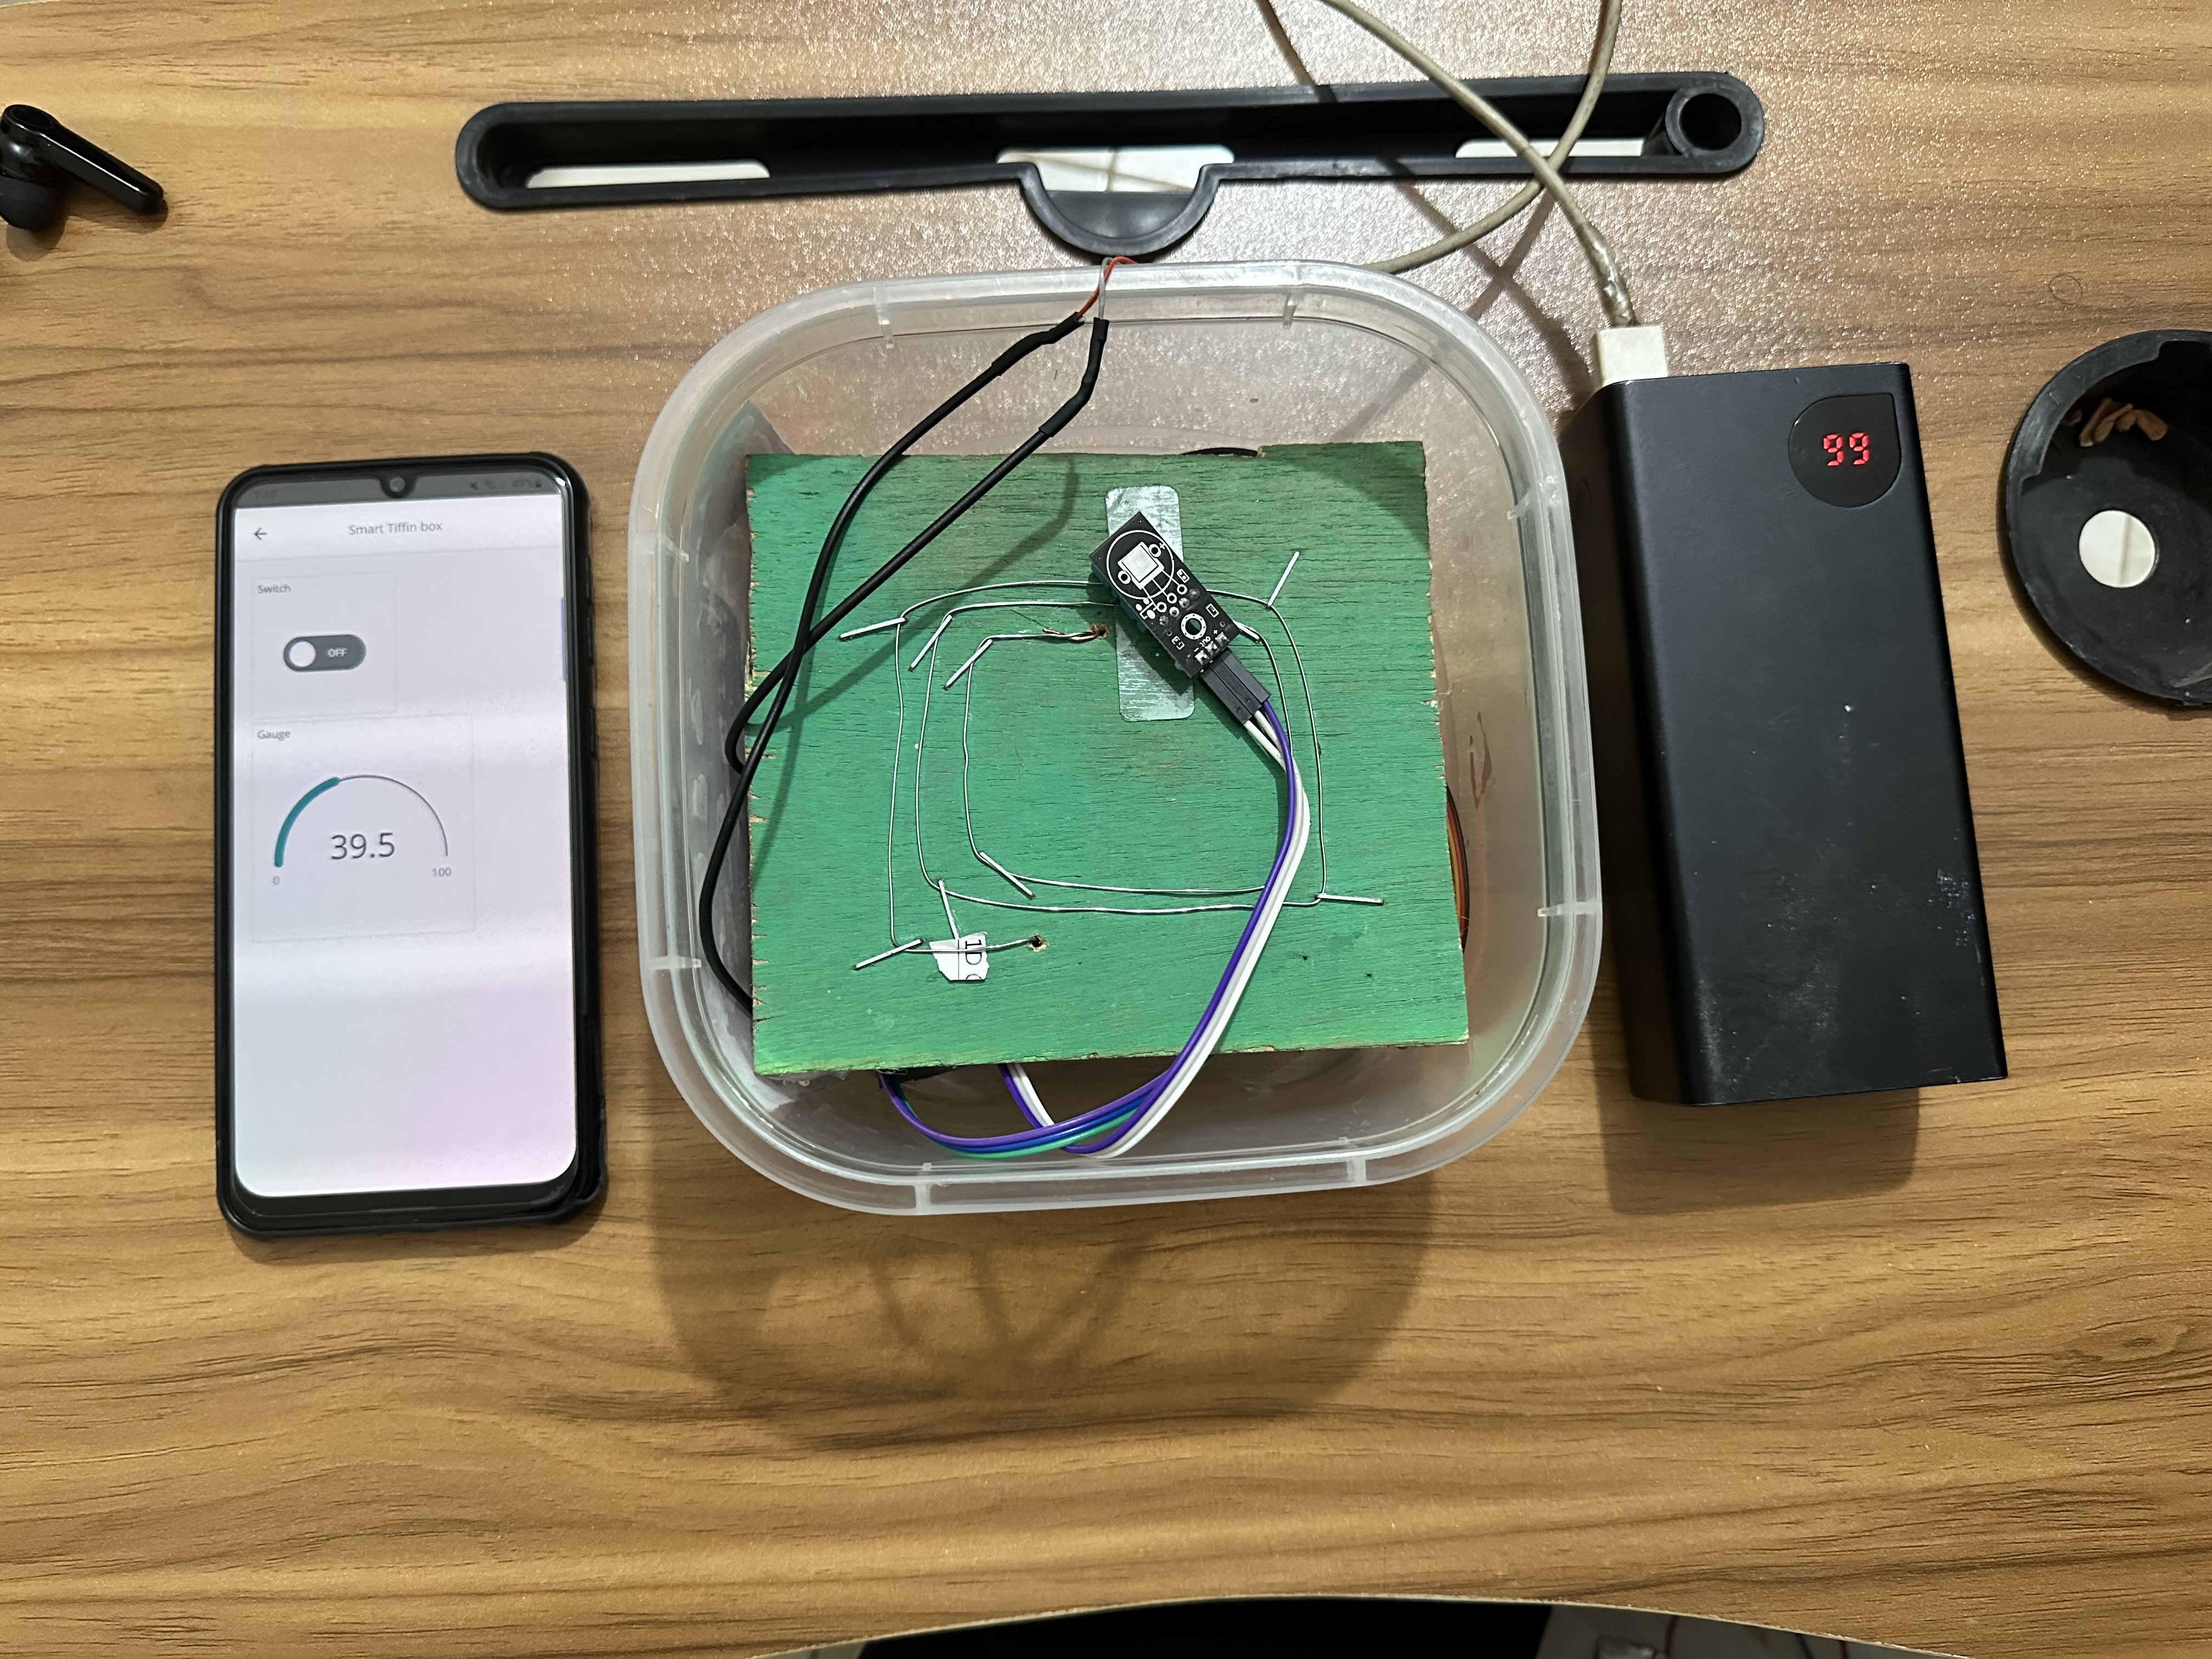
\includegraphics[width=0.5\textwidth, height=0.3\textwidth]{IMG_3508.jpg}}
\caption{Setup in Tiffin Box}
\label{fig}
\end{figure}

\begin{figure}[htbp]
\centerline{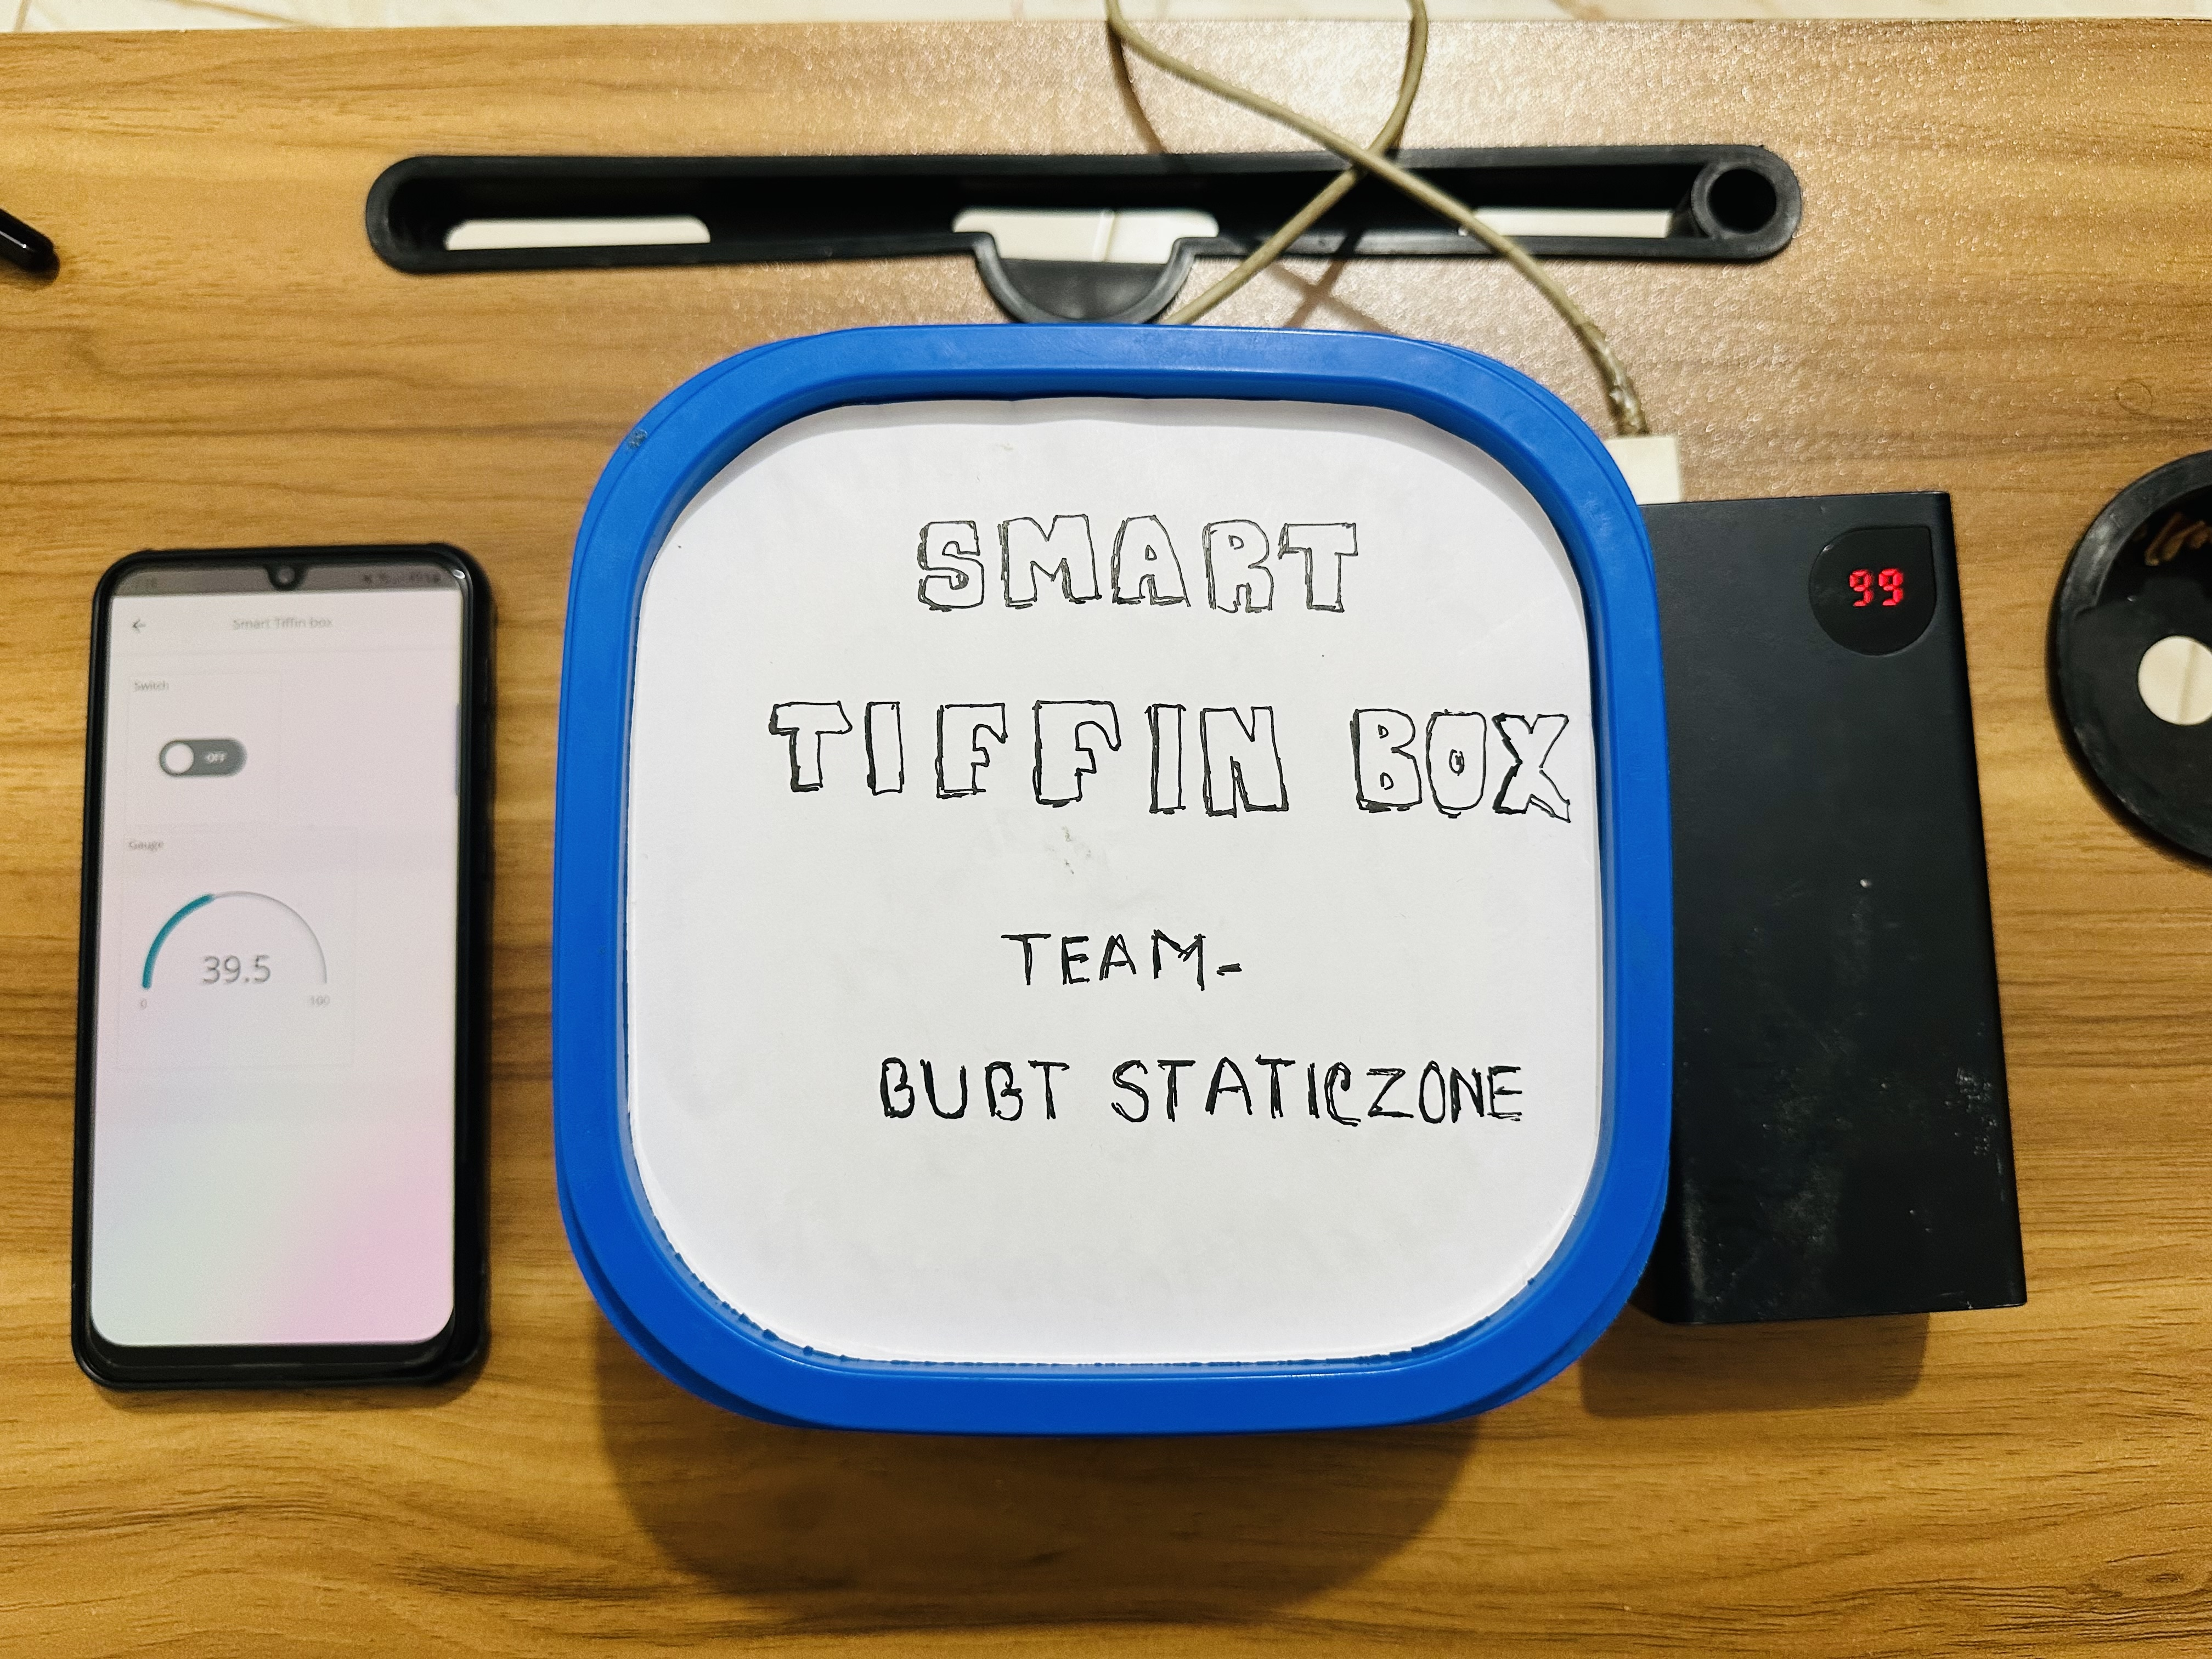
\includegraphics[width=0.5\textwidth, height=0.3\textwidth]{IMG_3511.jpg}}
\caption{Final Look}
\label{fig}
\end{figure}

\begin{figure}[htbp]
\centerline{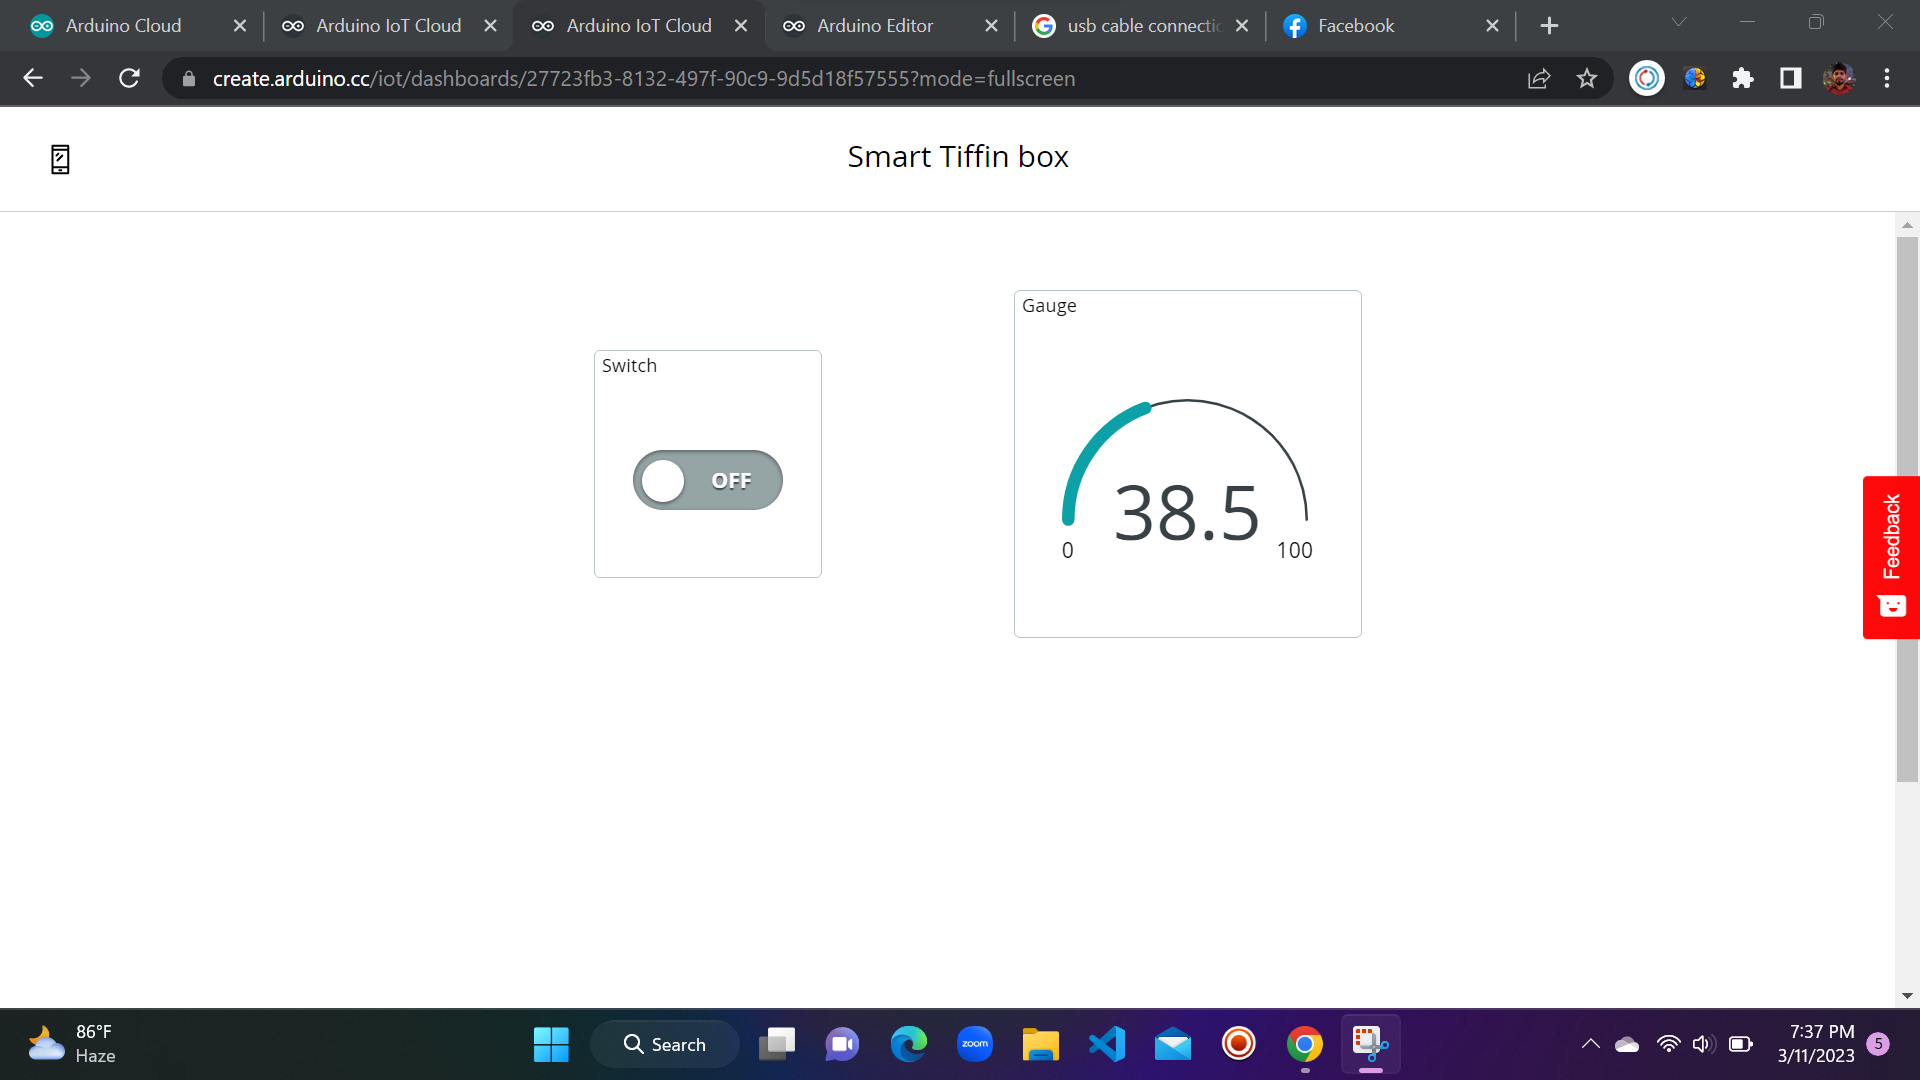
\includegraphics[width=0.5\textwidth, height=0.3\textwidth]{web.png}}
\caption{Web View}
\label{fig}
\end{figure}

\section{Advantages and Disadvantages}
\textbf{Advantages:\\}
Automated Temperature Control: SMART tiffin boxes come with automated temperature control, which helps maintain the temperature of the food items and keeps them fresh for a longer duration.\\
Food Safety: SMART tiffin boxes are equipped with sensors that monitor and record the temperature of the food items. This helps to ensure the safety of the food and reduces the risk of food contamination.\\
Convenience: With the help of an IoT based project, users can easily monitor and control the temperature of their tiffin box from any remote location. This makes it very convenient for users to monitor and control the temperature of their tiffin box from anywhere.\\
Reduced Wastage: SMART tiffin boxes help reduce wastage as they help maintain the freshness of the food items for a longer period of time. This helps in reducing the amount of food wastage. \\

\textbf{Disadvantages:\\}
High Cost: SMART tiffin boxes often come with a high price tag due to their unique technology and features. This can be a major disadvantage for people who are on a budget.\\
Limited Compatibility: SMART tiffin boxes may not be compatible with all types of IOT devices. This can limit the range of devices that can be used with the tiffin box.\\
Security Concerns: SMART tiffin boxes are connected to the internet and can be vulnerable to hacking and other security threats. This can be a major concern for users who want to keep their data secure.\\
Complex Setup: Setting up a SMART tiffin box requires some technical knowledge and can be a bit complicated for some users.\\
Limited Battery Life: SMART tiffin boxes tend to have limited battery life, which can be a major inconvenience for users who want to use the device for long periods of time.

\section{Application}
Tiffin boxes became the best way to carry home-cooked food in an era when hotels and restaurants were rare.  Tiffin Boxes are very versatile as they can be stored in a freezer, oven or dishwasher and the sturdy nature of steel means that it will never degrade. The main benefit of the Tiffin type carriers is to keep the foods apart, in a stable bag, to avoid soggy or smash your lunch until you can eat it.

% Create unordered list in LaTeX
\begin{itemize}
  \item It has most often been used by schoolchildren to take packed lunches, or a snack, from home to school.
  \item School teachers also carry their home cooked food to keep it warm.
  \item For someone who wishes to strictly move ahead with a diet, getting a tiffin box is an urgent requirement.
  \item People who work outside the home in factories, it became unfeasible to go home to lunch every day, thus it was necessary to have something to protect and transport a meal. They can easily keep their food using this tiffin box.
  \item Sometimes we arrange picnics and carry home cooked food, during this period we can carry our food in a tiffin box to keep the food warm and delicious.
  
\end{itemize}


\section{Conclusion}
IoT based SMART Tiffin Box for helps to keep warm food and live monitoring temperature of food. The System has high accuracy in fetching the live temperature of food. The IoT based SMART Tiffin box for the person who carries food from home people carry food from home for having good meal but after some time it loses temperature and test. This IOT device can warm food without having any hassle. 


\section{Future Scope}
IoT based SMART Tiffin Box for keeping food warm. In future we will add a weight scale for measuring the weight of food that will help the people who are suffering from diabetes and other diseases to have a fixed quantity of food. Also, it can help those people who are controlling their diet.


\section{References}
\begin{enumerate}
    \item https://www.designnest.com/mobile/Project/3a0l4b01a4rr/Smart-Lunch-Box
    \item https://www.kickstarter.com/projects/mysunnyside/smart-solar-powered-lunchbox-to-heat-and-chill-your-meal
\end{enumerate}
  
\section*{Apendix}
\textbf{Source Code:}
\begin{verbatim}
#include <DHT.h>
#include <DHT_U.h>
#include "thingProperties.h"
#include <Servo.h>
Servo servo;


#define DHTPIN 2
#define DHTTYPE DHT11
DHT dht(DHTPIN, DHTTYPE);


void powerOff();
void powerOn();

void setup() {
  Serial.begin(9600);
  dht.begin();
  delay(1500);
  
  servo.attach(4,2000,2400);

  // Defined in thingProperties.h
  initProperties();
  // int pos=0;

  // Connect to Arduino IoT Cloud
  ArduinoCloud.begin(ArduinoIoTPreferred
  Connection);
  
  setDebugMessageLevel(2);
  ArduinoCloud.printDebugInfo();
}

void loop() {
  ArduinoCloud.update();
  // Your code here
  
  float t = dht.readTemperature();
  // Your code here
  temperature = t;
  
  if(temperature > 37.0){
    powerOff();
    power = 0;
  
  }

}
bool control = false;
void onPowerChange()  {
  // Add your code here to act upon 
  Power change
  powerOn();
  powerOff();
  
}

void powerOn(){
  if(power == 1 /&& control == false){
    Serial.println("On");
    for(int pos=0;pos<=120;pos+=10){
      servo.write(pos);
      Serial.println(pos);
      
    }
    control = true;
  }
}

void powerOff(){
  if(power == 0 && control == true){
    Serial.println("Off");
    for(int pos=120;pos>=0;pos-=10){
      servo.write(pos);
      Serial.println(pos);
    }
    control = false;
  }
}
\end{verbatim}


\textbf{Wifi Connection Code:}
\begin{verbatim}
// Code generated by Arduino IoT Cloud,
DO NOT EDIT.

#include <ArduinoIoTCloud.h>
#include <Arduino_ConnectionHandler.h>

const char DEVICE_LOGIN_NAME[]= 
  "c5f30c04-caff-4911-8228-cfb183781dc1";

const char SSID[]= SECRET_SSID;    
const char PASS[]= SECRET_OPTIONAL_PASS;
const char DEVICE_KEY[]  = SECRET_DEVICE_KEY; 

void onPowerChange();

CloudTemperatureSensor temperature;
bool power;

void initProperties(){

  ArduinoCloud.setBoardId(DEVICE_LOGIN_NAME);
  ArduinoCloud.setSecretDeviceKey(DEVICE_KEY);
  ArduinoCloud.addProperty(temperature, READ, 
  ON_CHANGE, NULL);
  ArduinoCloud.addProperty(power, READWRITE, 
  ON_CHANGE, onPowerChange);

}

WiFiConnectionHandler ArduinoIoTPreferred
Connection(SSID, PASS);
\end{verbatim}

\end{document}
